\chapter{\babEmpat}
\label{bab:hasil}
% Semua angka pada bab ini dibaca dari app/results/*.json, app/results/external/*.json,
% app/results/tests/*.xml, app/results/api_latency.json, dan app/results/lighthouse/summary.json.
% Angka dapat berubah bila kode atau data dievaluasi ulang; lihat cap waktu dan hash pada berkas sumber.

\section{Lingkungan Implementasi dan Pengujian}
\label{sec:lingkungan-implementasi}

Takar dijalankan sebagai aplikasi web Vue.js dan API FastAPI dengan basis data SQLite satu berkas. Evaluasi yang tersimpan dijalankan pada Windows 11, Python 3.13.5, prosesor Intel Core i7-12700H, dan memori 31,7~GB. Pengukuran API memakai Uvicorn satu pekerja dan salinan basis data demo berukuran 30,9~MB; pada saat pengukuran terdapat 12 resep, 20 bahan, 80 produk katalog, dan 199.010 baris penjualan yang diimpor. Versi perangkat lunak, hash masukan, waktu, dan parameter eksperimen tersimpan dalam berkas JSON hasil, sehingga metrik pada bab ini adalah hasil lingkungan dan versi tersebut, bukan klaim kinerja universal.

Data pengembangan terdiri atas 49.894 baris IBM untuk pasangan menu dan 149.116 baris Maven untuk peramalan serta simulasi \textit{restock}. Kedua sumber ini adalah data sampel fiktif. Validasi eksternal memakai sumber yang berbeda sifatnya: transaksi Bread Basket dan ihelon, data seduhan konsumen UC Davis dan Batali, serta komposisi kafein menu Starbucks. Pemetaan produk luar ke resep aplikasi adalah asumsi penelitian; berkas pemetaan dan alasan setiap asumsi tersedia bersama kode.

\section{Implementasi Sistem}
\label{sec:implementasi}

Antarmuka menyediakan halaman masuk, beranda, katalog dan detail resep, formulir penyuntingan resep, kalkulator, panduan seduh, SOP dan checklist, inventaris, rekomendasi AI, diagnosis seduh, pengelolaan pengguna, serta data dan model. Kalkulator menampilkan kebutuhan per cangkir, total bahan, stok yang tersedia, peringatan, dan perbandingan dengan hasil linier. Ketika barista mencatat produksi, server menulis log produksi dan satu pergerakan pemakaian untuk setiap bahan hasil uraian BOM. Pengenal permintaan klien dipakai agar pengiriman ulang tidak mengurangi stok dua kali.

Resep arahan pembimbing ditanamkan sebagai basis pengetahuan dengan nilai yang berasal dari dokumen tersebut ditandai sumbernya. Angka yang tidak tersedia di arahan, misalnya ukuran gelas tertentu, stok awal, takaran subresep espreso, \textit{lead time}, dan kemasan pemasok, dinyatakan sebagai asumsi. Hak manajer, kepala barista, dan barista diterapkan pada API dan disajikan sesuai peran dalam navigasi. Tampilan ponsel menggunakan navigasi bawah, sedangkan layar lebih lebar memakai bilah samping. Gambar~\ref{fig:hasil-kalkulator} memperlihatkan contoh halaman kalkulator pada hasil \textit{build} yang diuji.

\begin{figure}[htbp]
\centering
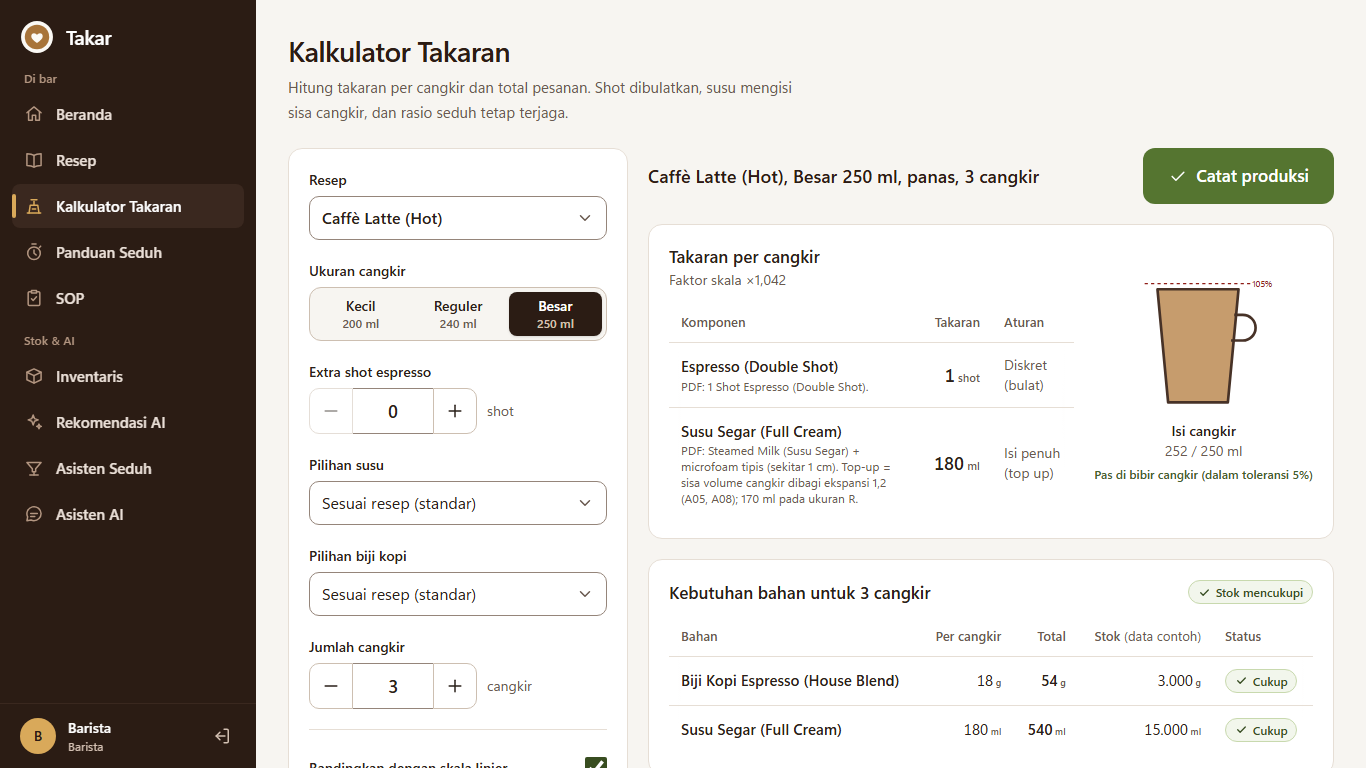
\includegraphics[width=.78\textwidth]{pic/results/screenshots/desktop/07-kalkulator-latte-besar-3-cangkir.png}
\caption{Tampilan Kalkulator Takaran Caffè Latte pada Pengujian Antarmuka}
\label{fig:hasil-kalkulator}
\end{figure}

Panduan Seduh dan Timer Shot menampilkan ilustrasi SVG yang bergerak mengikuti tahap resep aktif, misalnya aliran air pada V60, ekstraksi espreso, atau pengukusan susu. Judul langkah, waktu, target takaran, dan parameter tetap diambil dari data resep; animasi hanya membantu mengenali tindakan dan dapat dijeda, termasuk ketika perangkat meminta pengurangan gerak. Dari rekomendasi pasangan menu, tautan ``Pelajari resep'' membuka panduan bila produk saran mempunyai padanan resep aktif. Alur ini menghubungkan saran menu dengan prosedur yang dapat dipraktikkan, tetapi manfaatnya bagi pembelajaran barista masih memerlukan UAT.

\section{Hasil Pengujian Fungsional}
\label{sec:hasil-fungsional}

% sumber: results/tests/backend.xml, results/tests/e2e.xml, results/tests/blackbox_cases.csv
% sumber: results/tests/backend.xml dan results/tests/blackbox_cases.csv.
Berkas pengujian akhir mencatat 706 kasus \textit{pytest} backend dan 29 kasus \textit{end-to-end} Playwright, semuanya lulus tanpa kegagalan. Kasus antarmuka mencakup masuk dengan tiga peran, penolakan kata sandi keliru, hak akses barista, daftar dan detail resep, variasi kalkulator, pencatatan produksi, mutasi stok, checklist SOP, timer, rekomendasi AI, asisten lokal, animasi seduh, tautan dari saran pasangan ke panduan, serta tampilan ponsel. Berkas \texttt{blackbox\_cases.csv} menyimpan langkah, hasil yang diharapkan, hasil yang benar-benar terbaca pada layar, dan status tiap kasus. Jumlah kasus ini menyatakan cakupan suite otomatis saat berkas dihasilkan; ia tidak menggantikan uji penerimaan oleh barista kedai.

Pengujian layanan juga memeriksa permintaan tanpa token dan peran yang tidak berhak, validasi pesanan, serta transaksi stok. Skenario perhitungan V60 15~g menghasilkan air 225~ml dan target tuang 45, 130, serta 225~ml; pada dosis 20~g kebutuhan air menjadi 300~ml dan target kumulatif 60, 173,3, serta 300~ml. Hasil ini merupakan pemeriksaan terhadap aturan resep yang telah ditetapkan, bukan pengukuran rasa seduhan di lapangan.

\section{Hasil Evaluasi Penskalaan Resep}
\label{sec:hasil-penskalaan}

% sumber: results/scaling_eval.json (summary.methods, headline, parameters)
Grid evaluasi menghasilkan 525 pesanan efektif pada 12 resep jual. Grid itu meliputi tambahan sampai tiga \textit{shot}, sesuai batas masukan API; subset spesifikasi awal sampai dua \textit{shot} memuat 435 pesanan. Tabel~\ref{tab:hasil-penskalaan} membandingkan tiga metode pada 525 pesanan yang sama. Penskalaan berbasis batasan tidak menghasilkan \textit{shot} pecahan, luapan lebih dari 5\%, atau penyimpangan rasio lebih dari 0,2. Penskalaan linier mentah menghasilkan 240 pesanan dengan \textit{shot} pecahan dan 267 luapan; versi linier yang dibulatkan menghapus \textit{shot} pecahan, tetapi menghasilkan 282 luapan. Dengan kriteria H1 yang ditetapkan pada Bab~\ref{bab:pendahuluan}, H1 didukung pada grid ini.

\begin{table}[htbp]
\centering
\caption{Pelanggaran Penskalaan pada 525 Pesanan Uji}
\label{tab:hasil-penskalaan}
\small
\begin{tabular}{lrrr}
\toprule
Pemeriksaan & Berbasis batasan & Linier dibulatkan & Linier mentah \\
\midrule
\textit{Shot} pecahan & 0 & 0 & 240 \\
Luapan cangkir & 0 & 282 & 267 \\
Penyimpangan rasio & 0 & 0 & 0 \\
Ketelitian tidak praktis & 0 & 0 & 300 \\
Jumlah batch tidak konsisten & 0 & 0 & 183 \\
Peringatan kurang isi & 144 & 0 & 0 \\
\bottomrule
\end{tabular}
\end{table}

Nilai nol untuk \textit{shot} pecahan dan ketidaksesuaian jumlah batch pada metode berbasis batasan dijamin oleh aturan diskret dan perkalian takaran per cangkir; karena itu hasil tersebut diberi penanda \textit{by construction}. Selain itu, 144 pesanan berbasis batasan menerima peringatan kurang isi karena jumlah komponen pengisi berada di bawah batas minimum resep. Peringatan ini tidak masuk tiga kriteria H1, tetapi menunjukkan bahwa mencegah luapan saja belum menjamin semua minuman mencapai komposisi yang diinginkan. Pengujian sensorik dan keputusan barista dibutuhkan untuk menilai apakah pesanan seperti itu sebaiknya ditolak atau resepnya disesuaikan.

Gambar~\ref{fig:hasil-skala} memperlihatkan persentase pelanggaran yang dapat membedakan ketiga metode. Penyimpangan rasio bernilai nol pada semua metode di grid tersebut, sehingga tidak ditampilkan dalam grafik.
\begin{figure}[htbp]
\centering
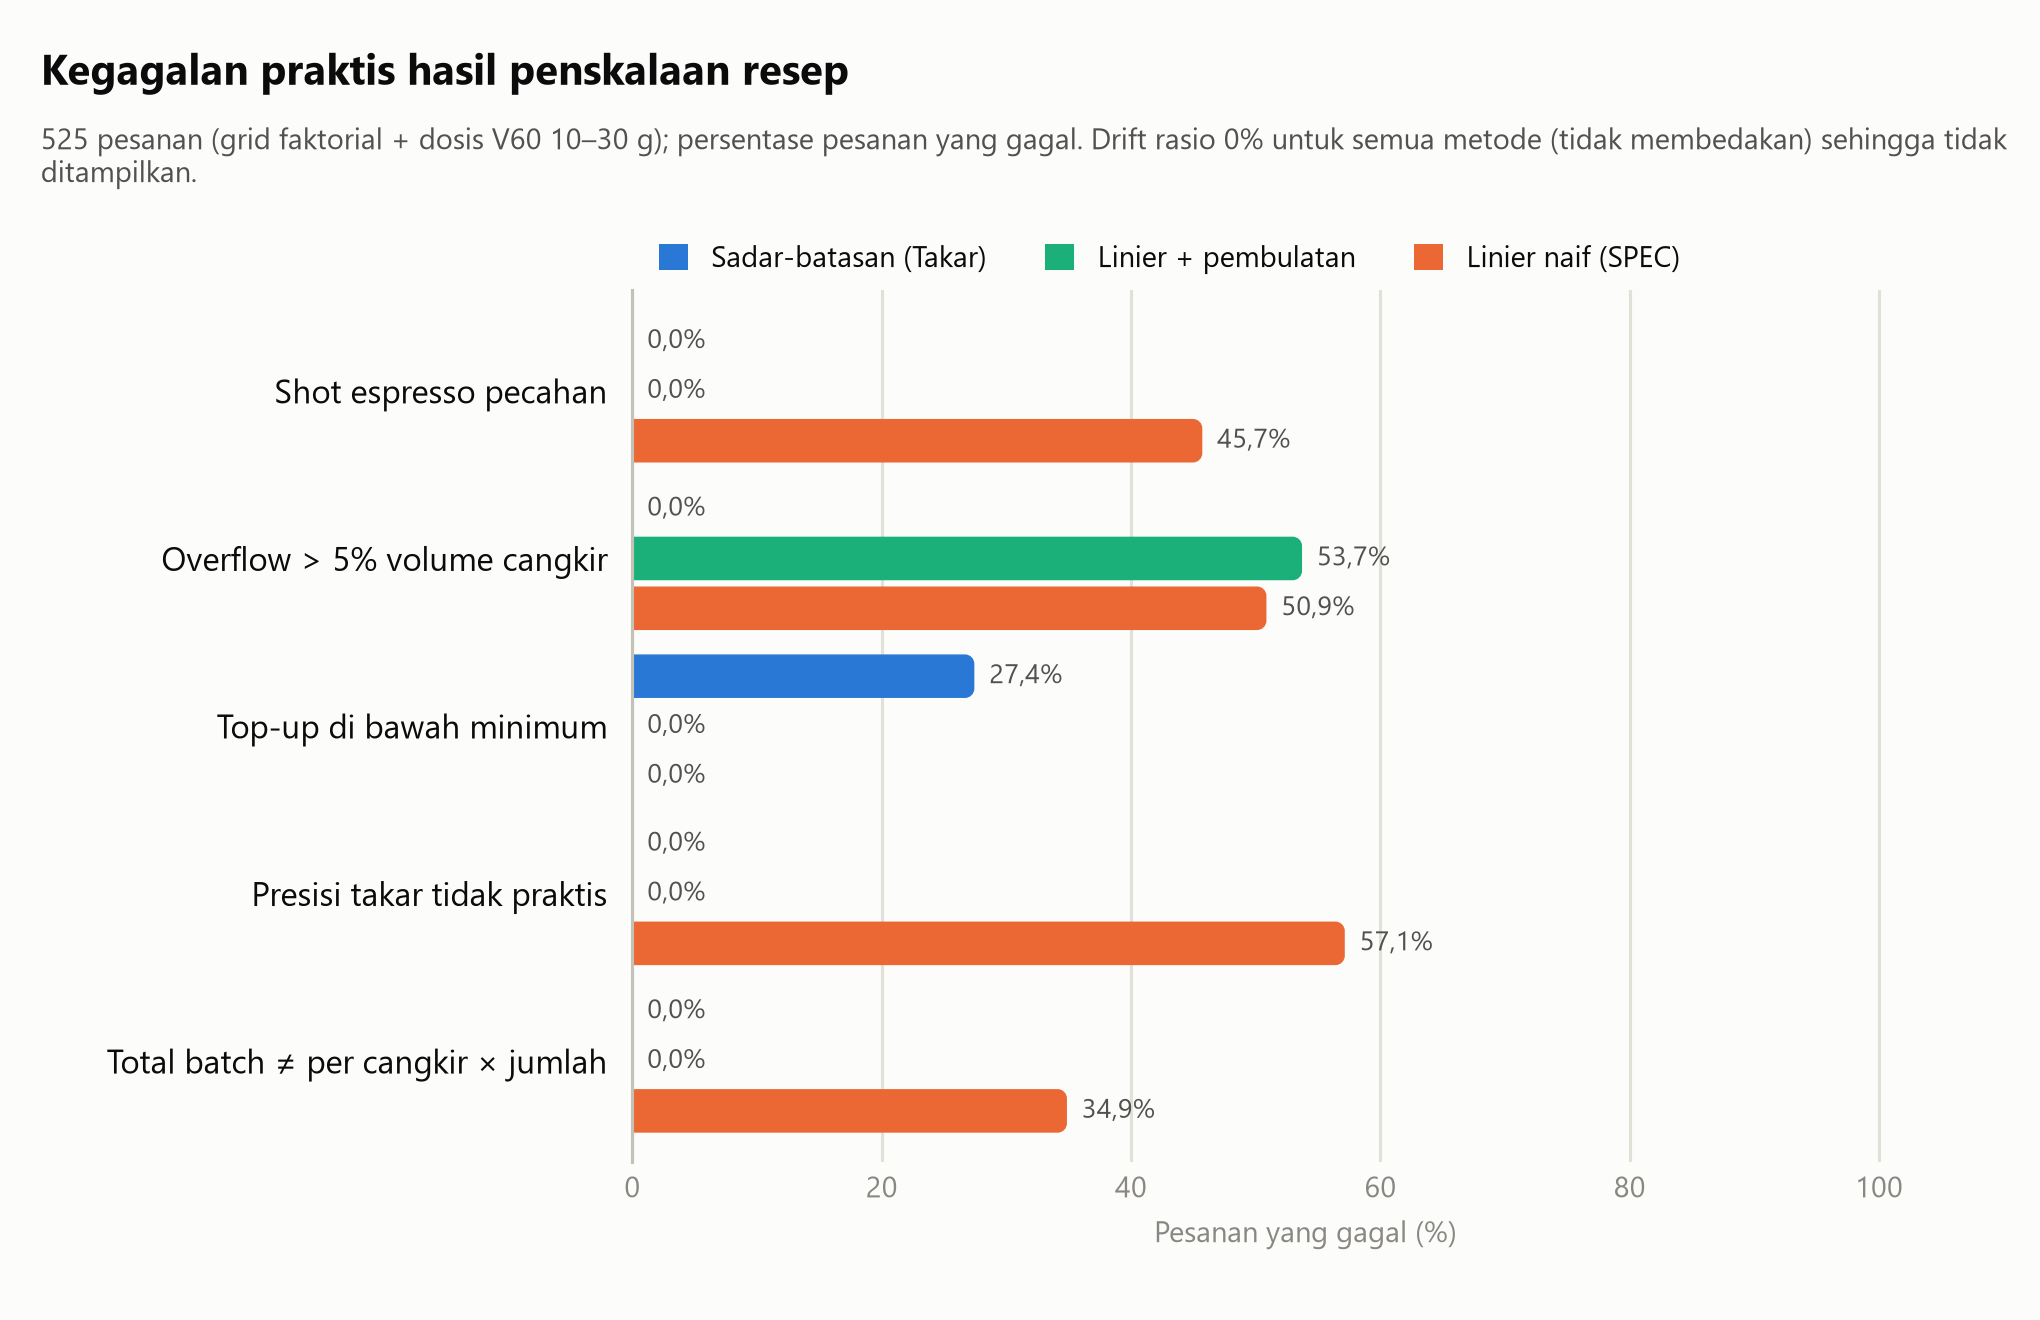
\includegraphics[width=.82\textwidth]{pic/results/figures/scaling_eval.png}
\caption{Kegagalan Praktis pada Grid Penskalaan Resep}
\label{fig:hasil-skala}
\end{figure}

% sumber: results/external/E5_scaling_starbucks.json (headline)
Validasi eksternal E5 memakai tujuh minuman berbasis espreso pada empat ukuran; kombinasi tiga ukuran bukan dasar per minuman menghasilkan 84 prediksi yang dikumpulkan lintas pilihan ukuran dasar. Proporsi hasil linier mentah yang berupa \textit{shot} pecahan adalah 84,5\%, sedangkan aturan diskret menghasilkan 0\% karena sifat konstruksinya. Tingkat kecocokan tepat terhadap jumlah \textit{shot} menu adalah 14,3\% untuk hasil linier mentah dan 58,3\% untuk aturan diskret dengan pembulatan setengah ke atas. Pengecualian ukuran mencapai 100\% karena tabel itu diisi langsung dari jumlah \textit{shot} menu; angka tersebut membuktikan kemampuan representasi, bukan akurasi prediksi. Hasil ini mendukung kebutuhan aturan diskret dan data pengecualian ukuran, tetapi satu menu jaringan di Amerika Serikat tidak mewakili semua kedai kopi.

\section{Hasil Evaluasi Rekomendasi Pasangan Menu}
\label{sec:hasil-pasangan}

% sumber: results/pairing_eval.json; results/external/E1_pairing_breadbasket.json
Pada data sampel fiktif IBM, periode uji 22--29 April 2019 menghasilkan 2.067 keranjang multi-item dan 4.260 kueri \textit{leave-one-out}. FP-Growth yang dipakai aplikasi, yaitu aturan dengan \textit{lift} lebih dari satu, mencapai HR@5 sebesar 0,4941 dan MRR@5 sebesar 0,2902. Popularitas mencapai HR@5 0,1324, sedangkan ko-okurensi mencapai 0,5134. Selisih HR@5 FP-Growth terhadap popularitas 0,3617 dengan selang kepercayaan (IK) \textit{bootstrap} 95\% [0,3402; 0,3839]. Dengan demikian, H2 didukung pada data pengembangan IBM, tetapi ko-okurensi sederhana justru lebih baik pada HR@5.

Pada 1.165 keranjang multi-item nyata Bread Basket, diperoleh 3.167 kueri uji. Tabel~\ref{tab:hasil-pasangan} menunjukkan bahwa HR@5 FP-Growth 0,5718 hanya sedikit di atas popularitas 0,5658. Selisih berpasangan 0,0060 mempunyai IK 95\% [-0,0028; 0,0147], sehingga H2 tidak didukung pada data nyata ini. Ko-okurensi mencapai HR@5 0,6021 dan MRR@5 0,4015, keduanya lebih tinggi daripada FP-Growth yang dipakai aplikasi. Nilai MRR@5 FP-Growth 0,3768 bahkan lebih rendah dari popularitas 0,3871; selisihnya -0,0103 dengan IK 95\% [-0,0199; -0,0005].

\begin{table}[htbp]
\centering
\caption{Kinerja Pasangan Menu pada Data Uji Bread Basket}
\label{tab:hasil-pasangan}
\begin{tabular}{lrrr}
\toprule
Metode & HR@1 & HR@5 & MRR@5 \\
\midrule
Popularitas & 0,2807 & 0,5658 & 0,3871 \\
Ko-okurensi & 0,2851 & 0,6021 & 0,4015 \\
FP-Growth (\textit{lift} $>1$) & 0,2674 & 0,5718 & 0,3768 \\
FP-Growth semua aturan (ablasi) & 0,2839 & 0,5851 & 0,3962 \\
\bottomrule
\end{tabular}
\end{table}

Ablasi tanpa saringan \textit{lift} meningkatkan HR@5 Bread Basket menjadi 0,5851, tetapi bukan metode yang disajikan aplikasi dan tidak dipakai untuk keputusan H2. Salah satu penyebab yang ditemukan adalah saringan \textit{lift} membuang 36 dari 83 aturan menuju Coffee pada periode latih, karena Coffee sendiri sangat populer. Dataset Bread Basket berasal dari satu toko roti-kafe Edinburgh dan lisensi unggahan paling awal tidak jelas; karena itu perbedaan ini menjadi peringatan tentang transfer model, bukan dasar untuk menyatakan seluruh aturan asosiasi tidak berguna.

Perbedaan antarmetode pada data nyata dan IK selisih berpasangan diringkas pada Gambar~\ref{fig:hasil-pasangan-eksternal}. Selang HR@5 FP-Growth dikurangi popularitas memotong nol, sedangkan selang HR@1 dan MRR@5 berada di bawah nol.
\begin{figure}[htbp]
\centering
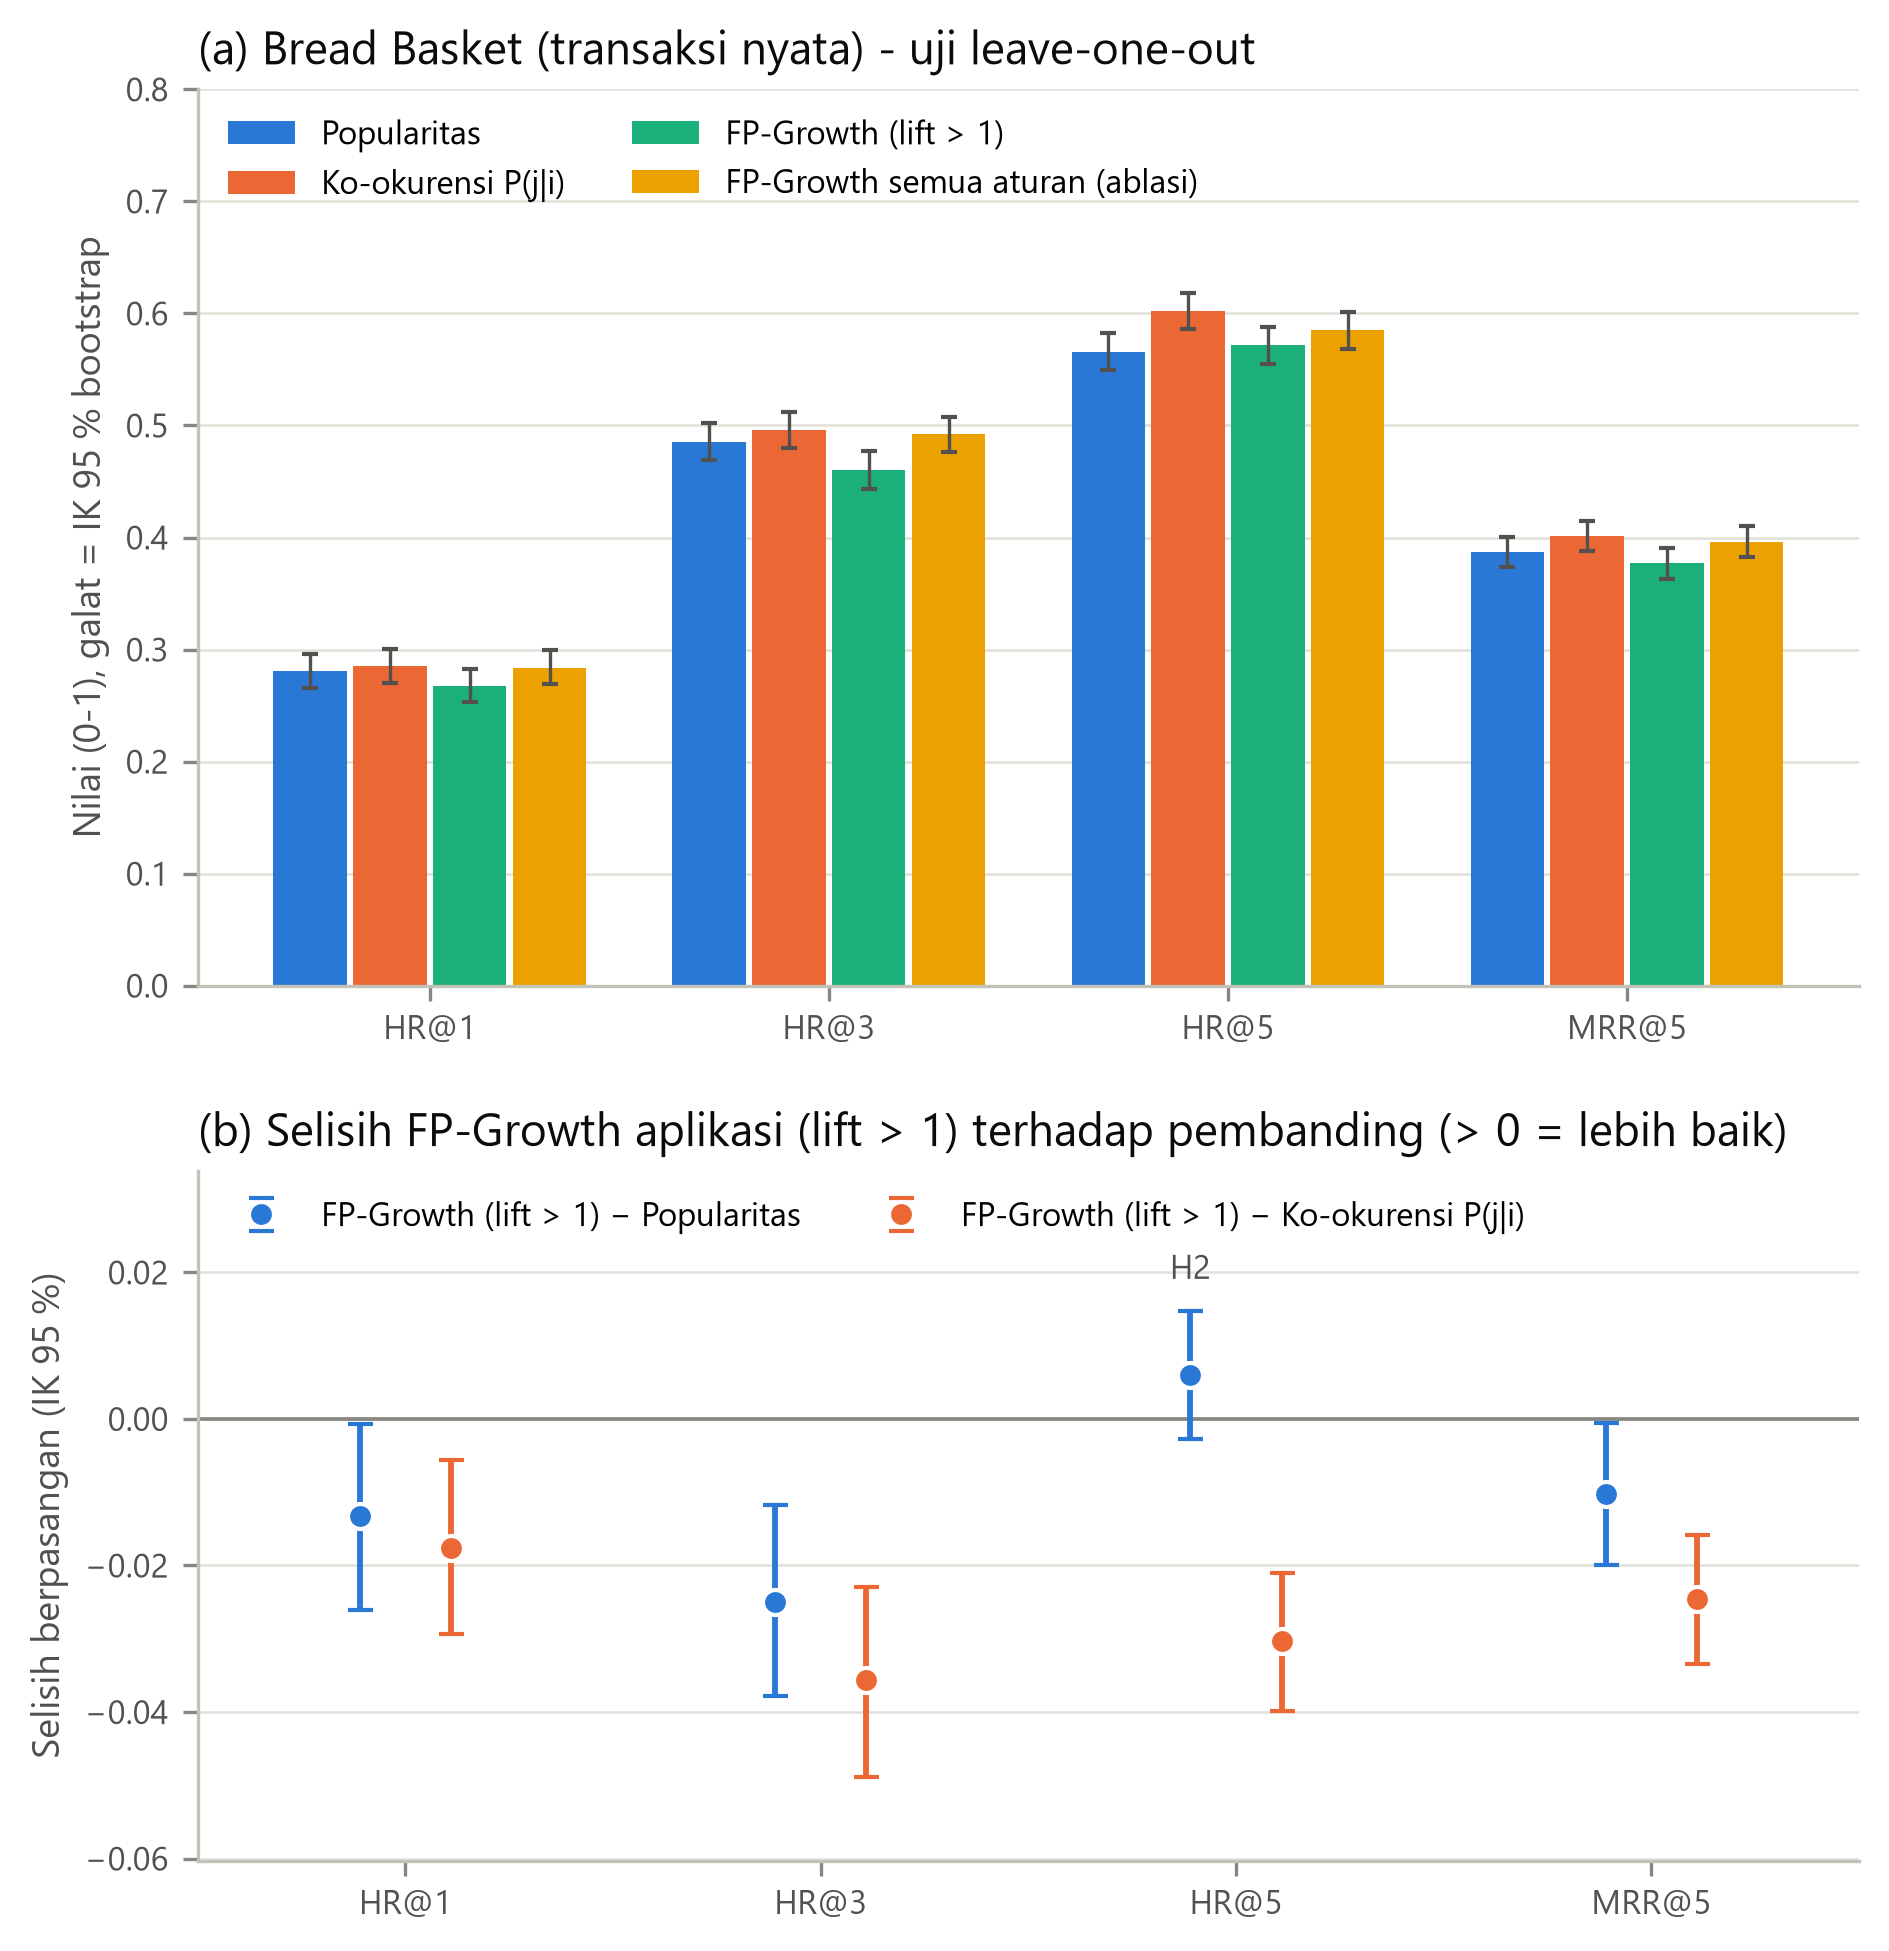
\includegraphics[width=.76\textwidth]{pic/results/figures/external_E1_pairing.png}
\caption{Kinerja Pasangan Menu dan Selisih Berpasangan pada Transaksi Bread Basket}
\label{fig:hasil-pasangan-eksternal}
\end{figure}

\section{Hasil Evaluasi Peramalan Permintaan}
\label{sec:hasil-peramalan}

% sumber: results/forecast_eval.json (data, protocol, overall)
Maven menyediakan 149.116 baris penjualan selama 181 hari, yang dibentuk menjadi 240 deret produk--outlet. Delapan origin mingguan dengan horizon tujuh hari menghasilkan 13.440 titik prediksi per metode. Tabel~\ref{tab:hasil-peramalan} menunjukkan bahwa \textit{gradient boosting} global memperoleh WAPE terendah, 0,3964, dibandingkan \textit{seasonal naive} 0,5381; model itu dipilih untuk aplikasi sebelum data validasi ihelon dinilai. Peramalan produk yang mempunyai pemetaan BOM juga diuraikan menjadi kebutuhan bahan, tetapi ketepatan pada bahan bergantung pada ketepatan pemetaan produk ke resep.

\begin{table}[htbp]
\centering
\caption{Perbandingan WAPE Peramalan pada Data Pengembangan Maven}
\label{tab:hasil-peramalan}
\begin{tabular}{lr}
\toprule
Model & WAPE \\
\midrule
\textit{Gradient boosting} global & 0,3964 \\
\textit{Simple exponential smoothing} & 0,4073 \\
Holt-Winters & 0,4161 \\
Rata-rata bergerak tujuh hari & 0,4266 \\
\textit{Seasonal naive} & 0,5381 \\
\textit{Naive} & 0,5389 \\
\bottomrule
\end{tabular}
\end{table}

% sumber: results/external/E2_forecast_ihelon.json (h3)
Validasi E2 memakai 3.636 cangkir nyata dari satu mesin penjual kopi, delapan minuman, dan delapan origin uji mingguan. Model terpilih mempunyai WAPE per minuman 0,6582 versus \textit{seasonal naive} 0,7125. Selisih -0,0542 ber-IK 95\% [-0,1145; 0,0159], sehingga penurunan estimasi titik belum meyakinkan. Pada total harian yang diramal langsung, WAPE model terpilih 0,3862 justru lebih tinggi daripada \textit{seasonal naive} 0,2646; selisih 0,1216 ber-IK [0,0527; 0,1897]. Maka H3 tidak didukung pada validasi nyata, meskipun model yang sama unggul pada data pengembangan fiktif. Hasil eksploratif model Holt-Winters pada seri per minuman tidak dipakai mengganti keputusan H3 karena model itu dipilih sesudah jendela uji dilihat.

Gambar~\ref{fig:hasil-forecast-eksternal} menampilkan WAPE setiap model pada seri per minuman ihelon. Grafik ini membantu membedakan peringkat eksploratif dari pengujian H3 yang memakai model terpilih sebelumnya.
\begin{figure}[htbp]
\centering
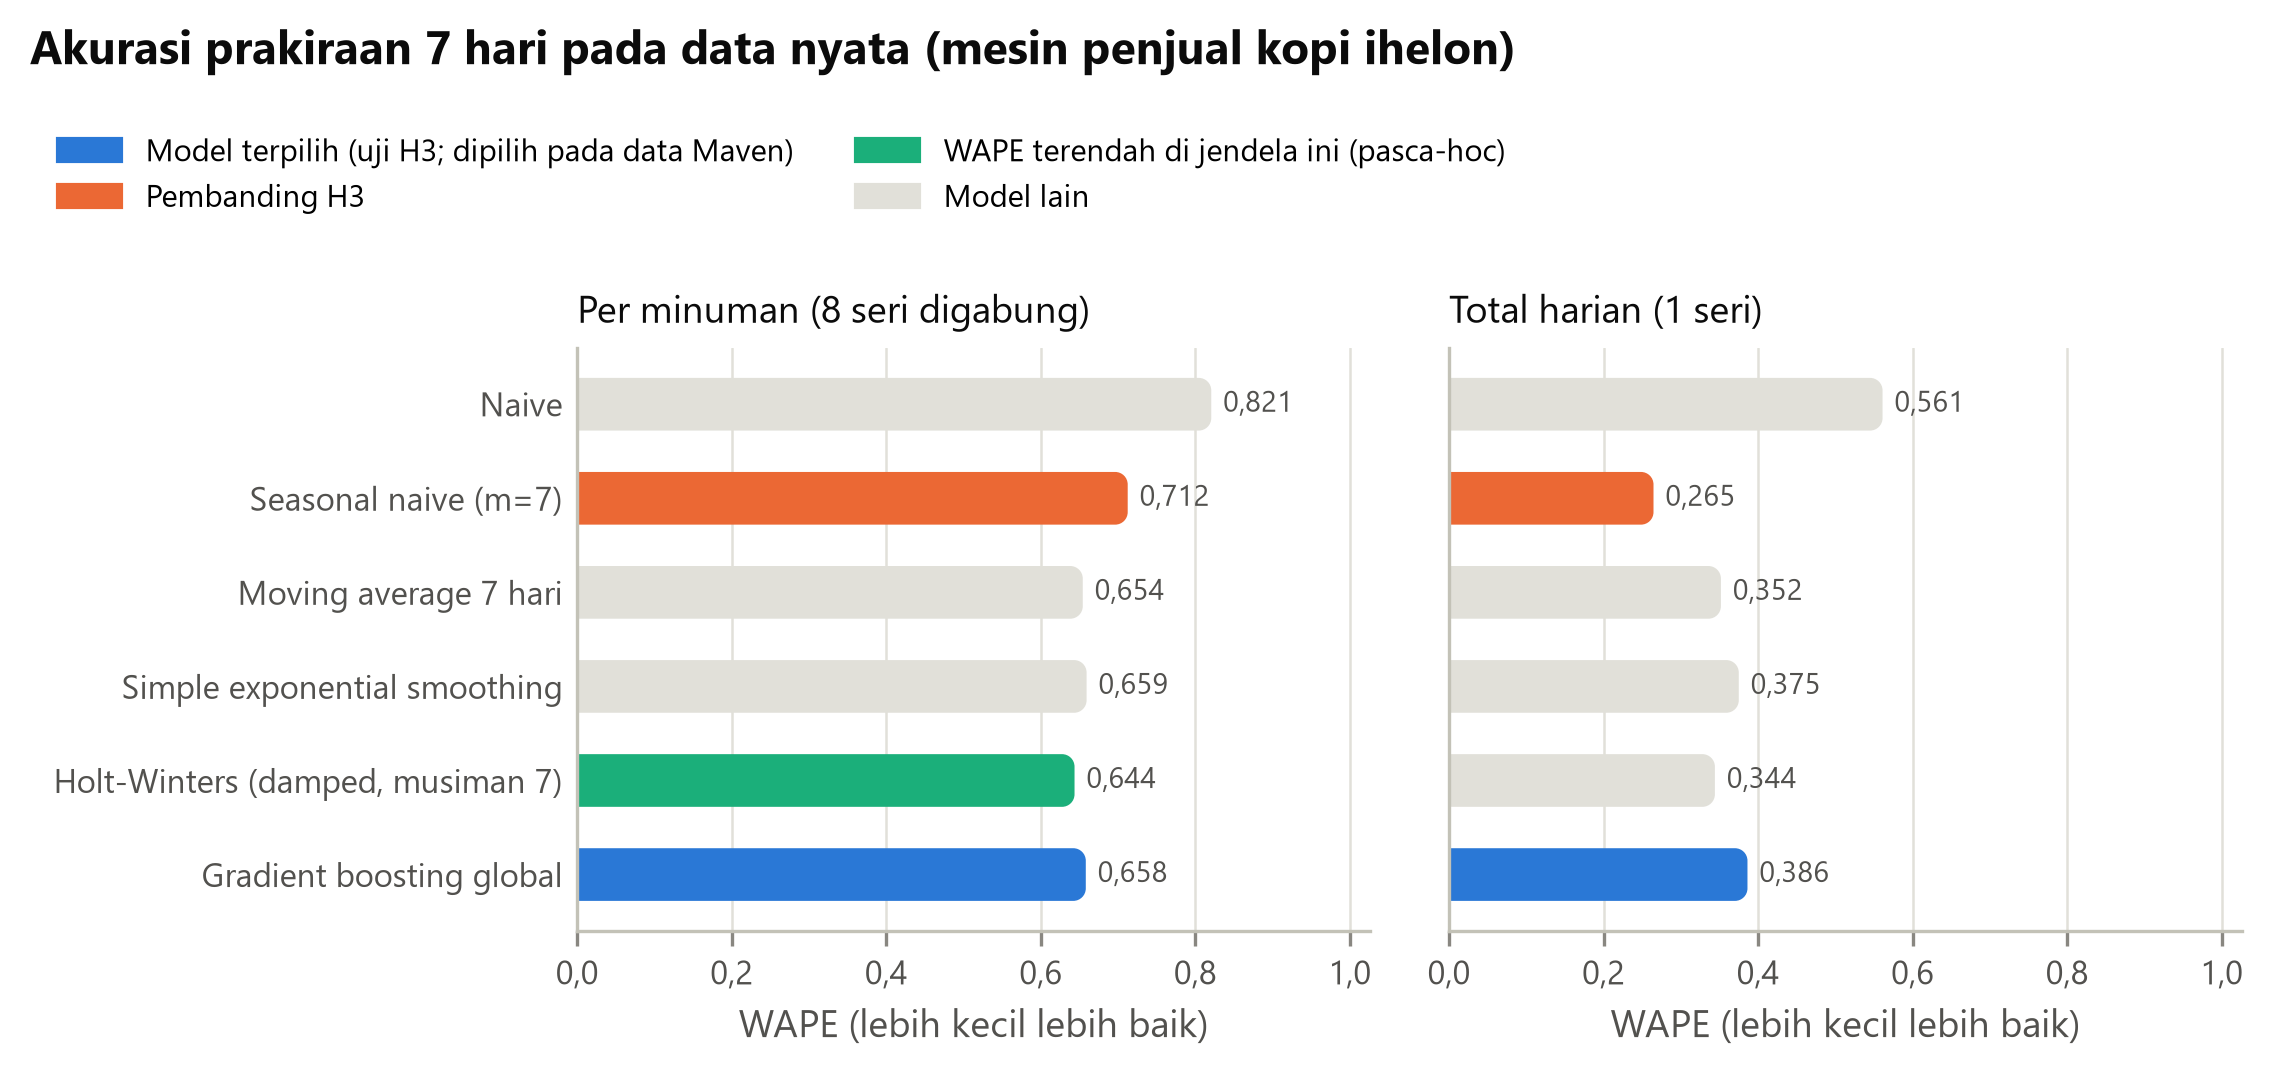
\includegraphics[width=.82\textwidth]{pic/results/figures/external_E2_wape_by_model.png}
\caption{WAPE Peramalan per Minuman pada Data Nyata ihelon}
\label{fig:hasil-forecast-eksternal}
\end{figure}

\section{Hasil Simulasi Rekomendasi \texorpdfstring{\textit{Restock}}{Restock}}
\label{sec:hasil-restock}

% sumber: results/restock_eval.json (summary, data)
Pada replay 56 hari data sampel fiktif Maven untuk 12 bahan, kebijakan tingkat sasaran berbasis prakiraan mencapai \textit{fill rate} rata-rata 0,9748 dan 60 hari kehabisan stok jika dijumlahkan lintas bahan. ROP statis mencapai 0,8173 dan 212 hari, sedangkan tingkat par mencapai 0,7138 dan 210 hari. Rata-rata stok yang dipegang kebijakan prakiraan 3,70 hari permintaan, lebih tinggi daripada ROP statis 2,55 hari. Dengan demikian, kenaikan layanan pada eksperimen ini mempunyai konsekuensi stok tertahan yang perlu dinilai bersama risiko bahan basi dan biaya kedai nyata.

% sumber: results/external/E3_restock_ihelon.json (summary, h4, ablation)
Validasi E3 mengubah transaksi ihelon menjadi permintaan tiga bahan demo. Pada replay 56 hari, kebijakan prakiraan mencapai \textit{fill rate} rata-rata 0,9605 dan 17 hari kehabisan stok, sedangkan ROP statis 0,7900 dan 47 hari. H4 didukung untuk perbandingan yang ditetapkan, dengan selisih \textit{fill rate} 0,1706. Akan tetapi, tingkat sasaran statis dengan struktur pemesanan yang sama sudah mencapai 0,8633; selisih 0,0972 terhadap kebijakan prakiraan memisahkan manfaat tingkat yang berubah dari manfaat struktur. Ketika struktur sama dan hanya model prakiraan diganti, rata-rata bergerak tujuh hari mencapai 0,9871 dan \textit{seasonal naive} 0,9671, keduanya di atas model terpilih 0,9605. H4 karenanya mendukung kebijakan dinamis pada skenario ini, bukan superioritas model \textit{machine learning}. Seluruh hasil bergantung pada \textit{lead time}, stok awal, dan ukuran kemasan yang merupakan data contoh.

Gambar~\ref{fig:hasil-restock-eksternal} memperlihatkan \textit{fill rate} per bahan dan per kebijakan. Perbedaan antarbahan menegaskan bahwa rata-rata tiga bahan tidak boleh dibaca sebagai jaminan tingkat layanan setiap bahan.
\begin{figure}[htbp]
\centering
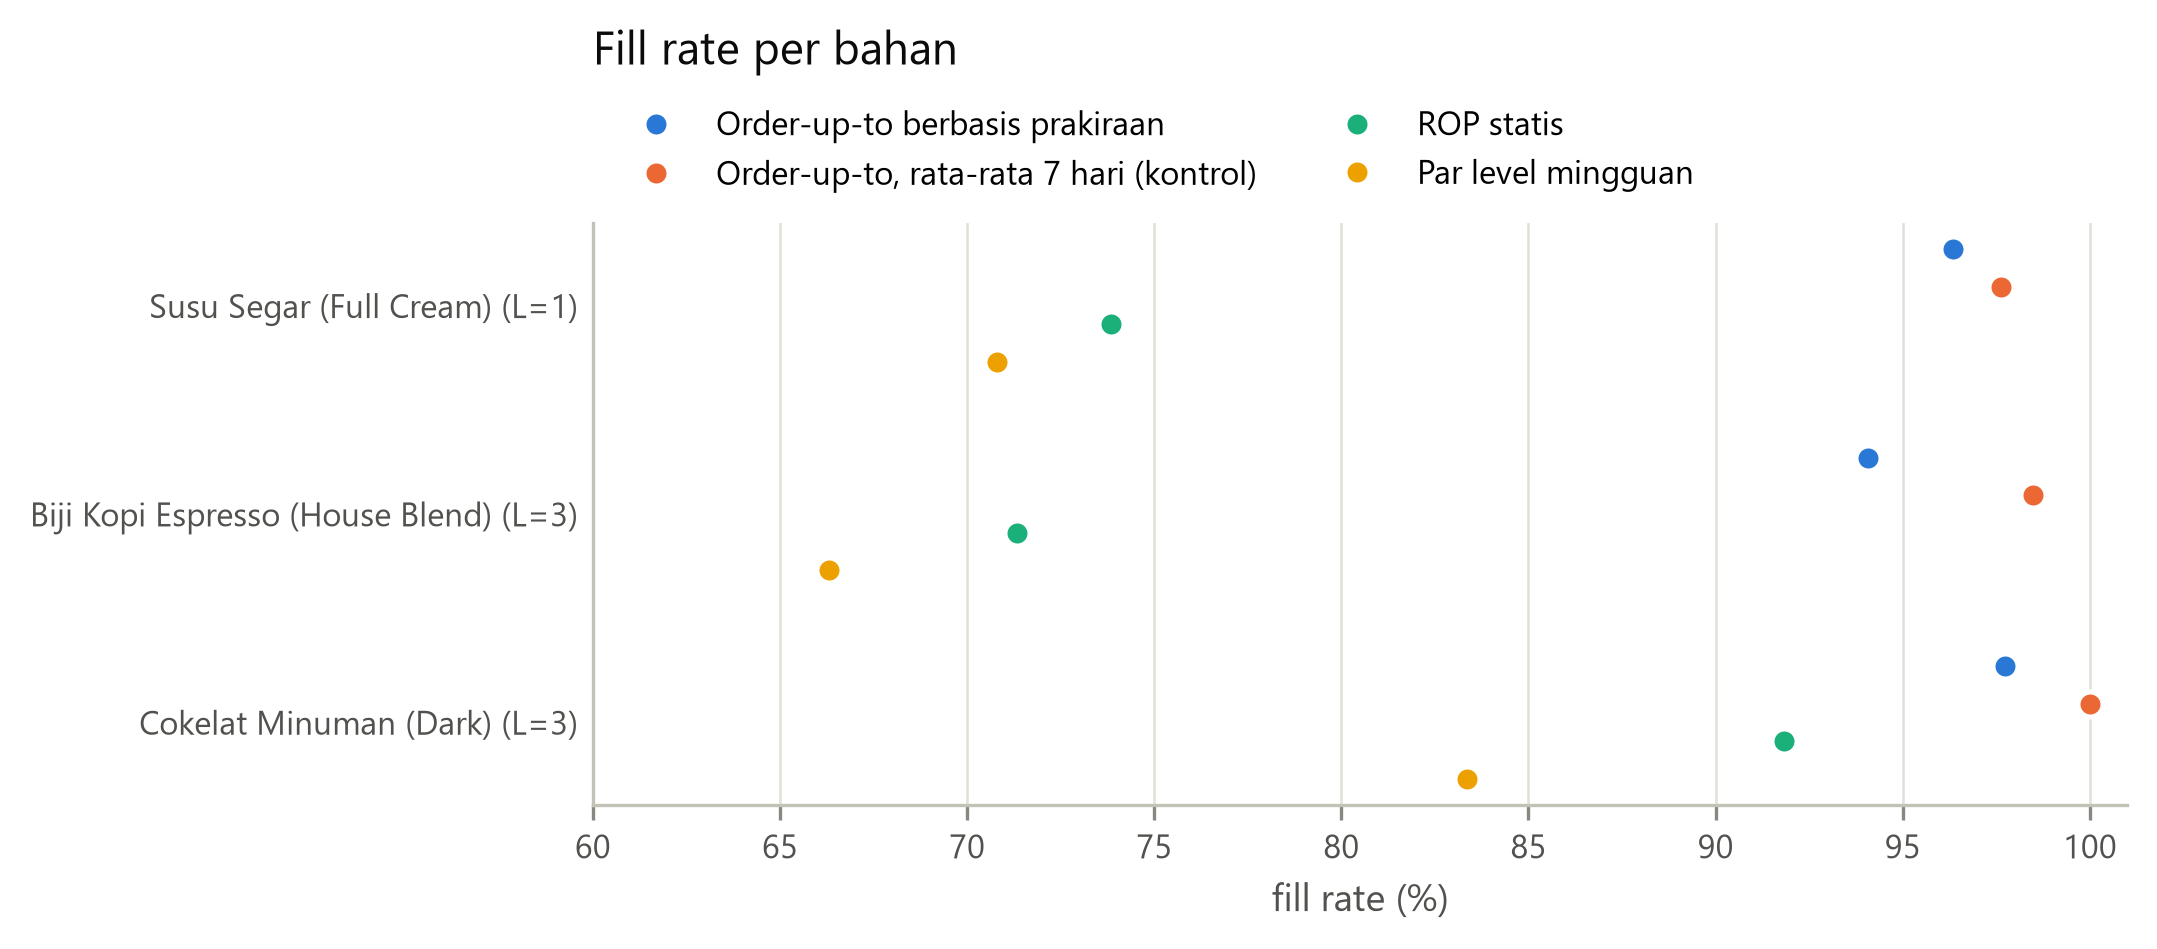
\includegraphics[width=.82\textwidth]{pic/results/figures/external_E3_fill_rate.png}
\caption{Tingkat Pemenuhan Permintaan Bahan pada Replay ihelon}
\label{fig:hasil-restock-eksternal}
\end{figure}

\section{Hasil Pengujian Sistem Pakar}
\label{sec:hasil-sistem-pakar}

% sumber: results/external/E4_expert_validation.json
Validasi E4 memakai 3.186 penilaian konsumen atas 162 seduhan; satu seduhan dengan EY di atas batas fisik ditolak, sehingga 3.164 penilaian atas 161 seduhan dapat dianalisis. Pada seduhan yang mempunyai massa minuman terukur, rumus EY mesin sama dengan nilai dataset sampai galat maksimum sekitar $5\times10^{-9}$ poin persentase. Ini memeriksa ketepatan perhitungan, bukan ketepatan diagnosis rasa. Basis aturan yang dipakai berisi 64 aturan.

Di antara penilaian \textit{just-about-right} yang bukan kategori pas pada seduhan yang ditandai lemah atau kuat oleh sistem, 820 dari 1.067 penilaian sesuai arah diagnosis, yaitu 76,9\% (IK 95\% [73,8\%; 80,0\%]). Kesepakatan berbeda menurut kelas: 89,5\% untuk lemah dan 60,7\% untuk kuat. Rerata kesukaan seduhan di dalam kotak \textit{Golden Cup} 5,812, sedangkan di luar 5,854; selisih -0,042 ber-IK 95\% [-0,233; 0,145]. Karena selang ini memuat nol dan preferensi konsumen bervariasi, sistem tidak menganggap kotak itu sebagai jaminan kesukaan.

Pada 27 resep eksperimen Batali, perbandingan arah koreksi yang dapat dinilai terhadap kotak acuan menunjukkan 26 dari 34 pasangan searah untuk tuas ekstraksi dan 12 dari 12 untuk tuas kekuatan. Sejumlah pasangan tidak menghasilkan saran tuas karena sudah berada pada pita target atau dibatasi fakta lain. Penelitian ini hanya membandingkan arah perubahan parameter yang diamati; ia tidak membuktikan bahwa semua saran sistem akan memperbaiki rasa bila diterapkan oleh barista pada bahan dan peralatan lain.

Sebaran TDS dan EY seduhan UC Davis terhadap kotak teknis ditunjukkan pada Gambar~\ref{fig:hasil-kendali-seduh}. Titik di dalam kotak adalah klasifikasi teknis, bukan label kesukaan peserta.
\begin{figure}[htbp]
\centering
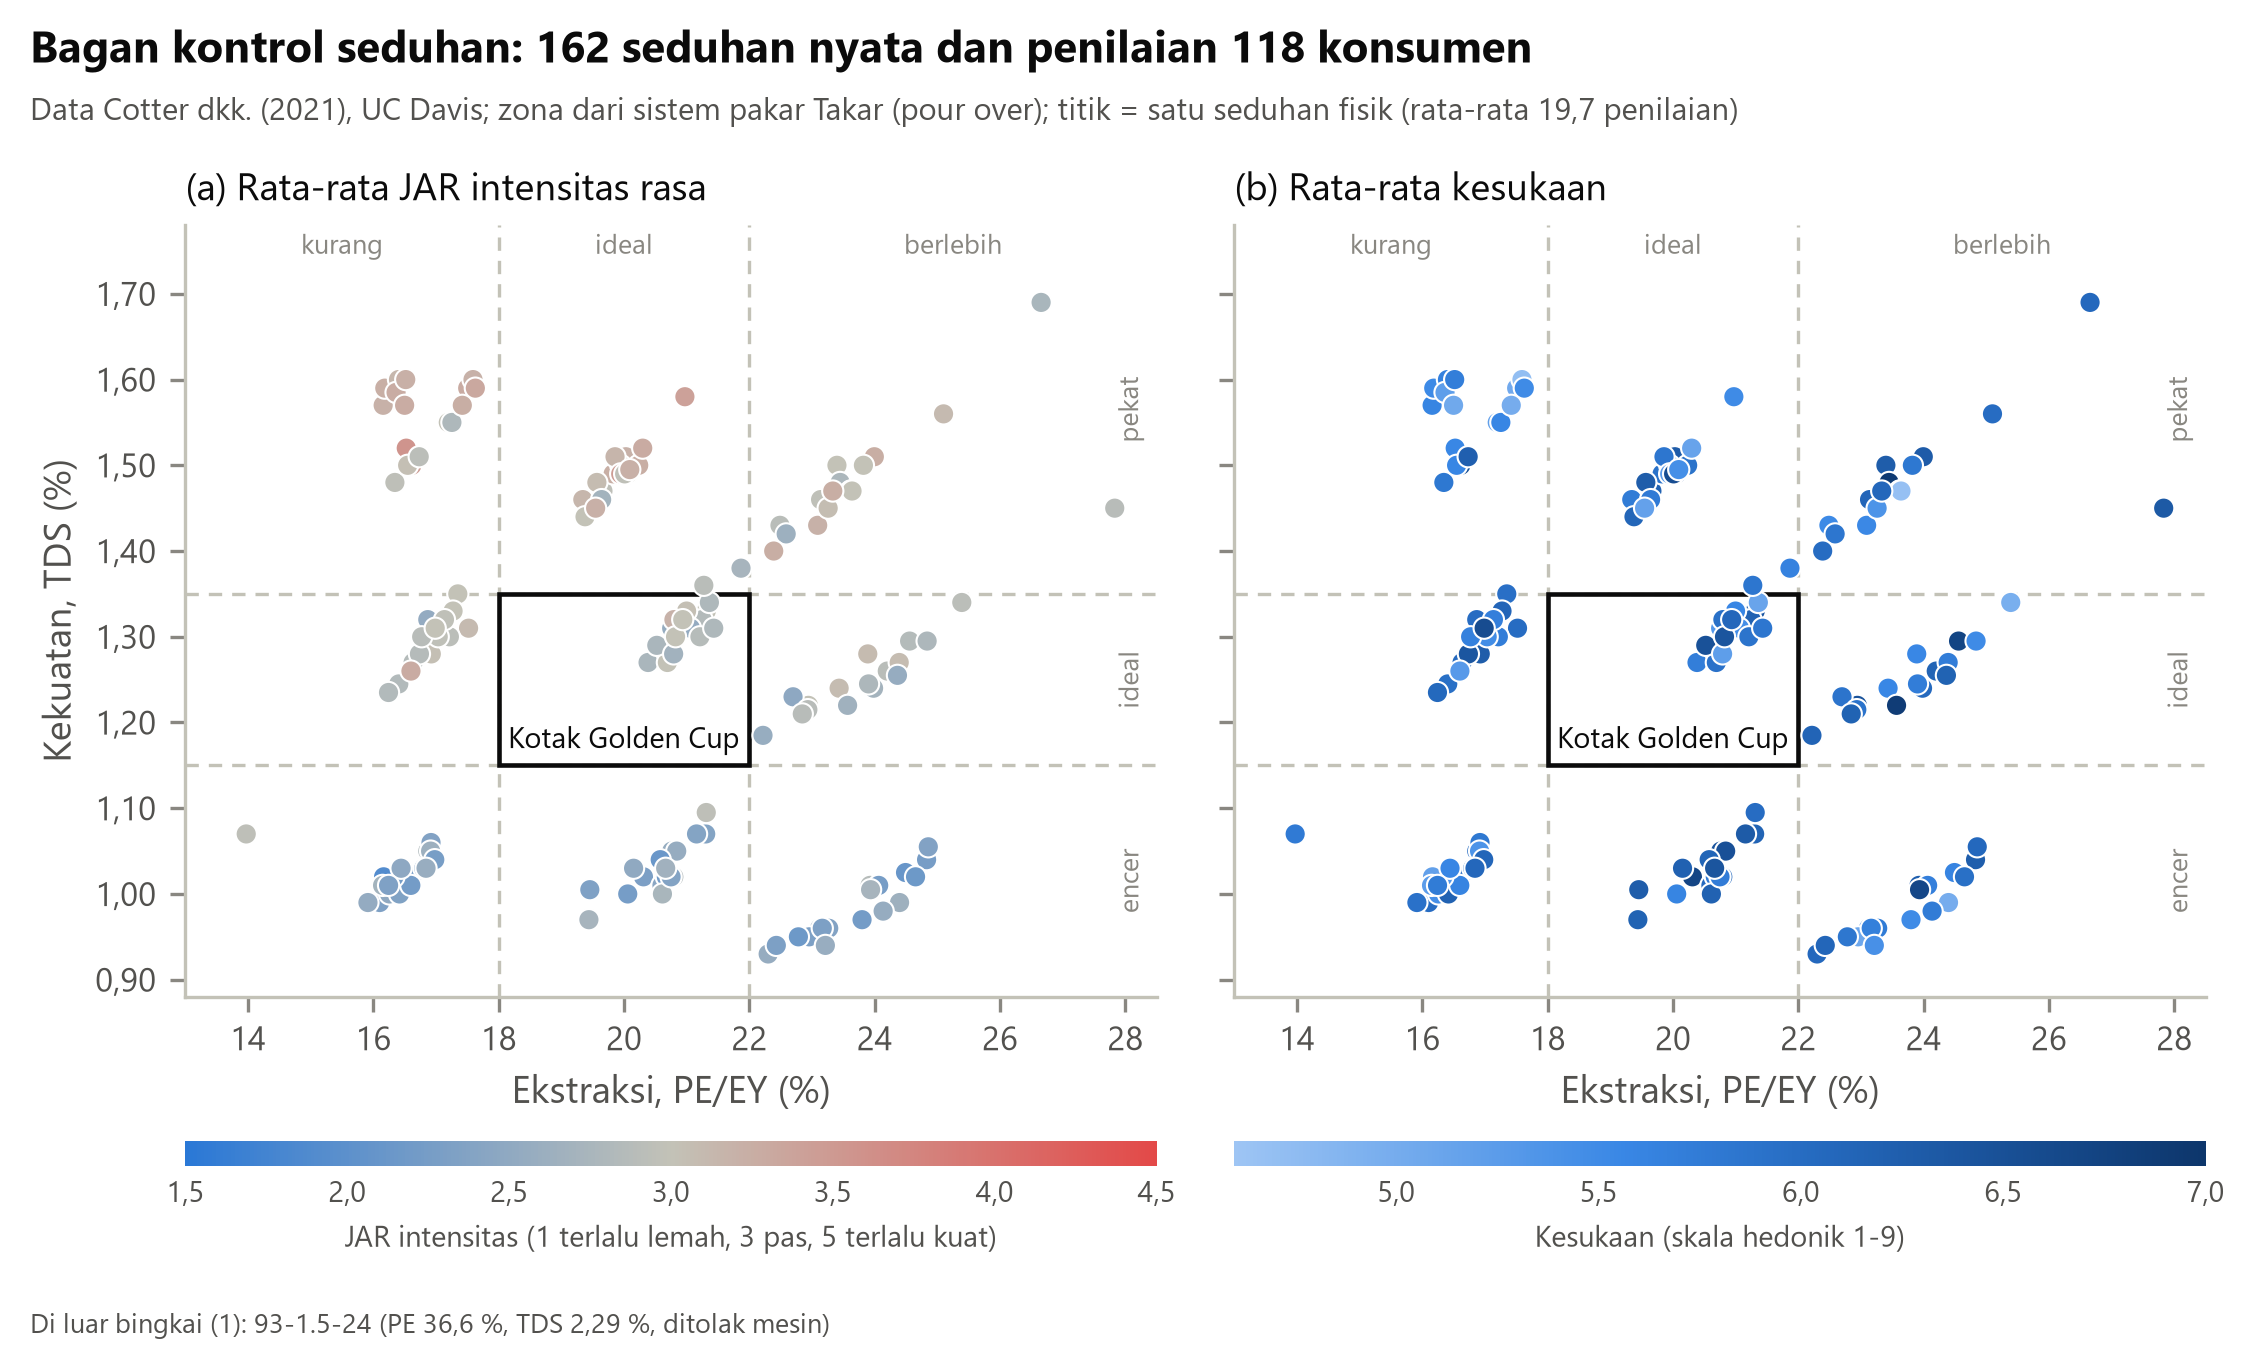
\includegraphics[width=.82\textwidth]{pic/results/figures/external_E4_control_chart.png}
\caption{Sebaran Seduhan Nyata pada Bagan Kendali Seduh}
\label{fig:hasil-kendali-seduh}
\end{figure}

\section{Hasil Evaluasi Asisten Barista AI}
\label{sec:hasil-asisten}

% sumber: results/assistant_eval.json (gabungan 420 jawaban, penilai versi 2.1).
Tolok ukur internal memuat 60 pertanyaan yang dibagi menjadi 14 fakta resep, 12 prosedur/SOP, 10 perhitungan, delapan diagnosis, enam stok, dan 10 pertanyaan di luar cakupan. Empat kondisi yang ditetapkan pada Bab~\ref{bab:metode} menghasilkan tujuh varian karena pencarian BM25 tidak memerlukan model dan tiga kondisi lain dijalankan pada Gemma 4 E4B serta E2B; totalnya 420 jawaban. Setelah kegagalan pemilihan alat pada percobaan awal ditemukan, hanya 120 jawaban kondisi RAG dengan alat dijalankan ulang pada router yang diperbaiki. Penggabungan dengan 300 jawaban kondisi lain memeriksa kesamaan hash tolok ukur dan basis data, lalu seluruh jawaban dinilai ulang oleh penilai versi 2.1. Suhu model ditetapkan nol dan \textit{seed} 42. Tabel~\ref{tab:hasil-asisten} melaporkan akurasi isi pada pertanyaan yang sama, akurasi yang juga mensyaratkan pemilihan alat dan argumen benar, serta latensi median seluruh pipeline.

\begin{table}[htbp]
\centering
\caption{Hasil Tolok Ukur Internal Asisten pada 60 Pertanyaan per Varian}
\label{tab:hasil-asisten}
\small
\begin{tabular}{llrrrr}
\toprule
Kondisi & Model & \shortstack{Akurasi\\isi (\%)} & \shortstack{Terverifikasi\\alat (\%)} & \shortstack{Mode\\LLM} & \shortstack{Latensi\\p50 (detik)} \\
\midrule
BM25 saja & -- & 55,0 & 55,0 & 0 & 0,027 \\
Tanpa konteks & E4B & 15,0 & 10,0 & 60 & 8,123 \\
RAG & E4B & 55,0 & 55,0 & 48 & 1,721 \\
RAG + alat & E4B & 95,0 & 95,0 & 26 & 0,175 \\
Tanpa konteks & E2B & 6,7 & 6,7 & 60 & 4,930 \\
RAG & E2B & 53,3 & 53,3 & 47 & 1,160 \\
RAG + alat & E2B & 93,3 & 93,3 & 26 & 0,150 \\
\bottomrule
\end{tabular}
\end{table}

Pencarian BM25 menempatkan rujukan benar pada peringkat pertama dalam 73,81\% dari 42 pertanyaan yang memiliki rujukan, pada tiga teratas dalam 85,71\%, dan pada lima teratas dalam 88,10\%; MRR-nya 0,7944. Akurasi pencarian saja 55,0\% pada seluruh 60 pertanyaan sudah mencakup penolakan pertanyaan di luar cakupan oleh gerbang aturan. Tabel~\ref{tab:hasil-asisten-kategori} menunjukkan bagian yang menyumbang perubahan E4B. Fakta resep sudah benar 14/14 pada RAG tanpa alat, sedangkan prosedur benar 9/12; keduanya tidak berubah setelah alat ditambahkan. Perhitungan, diagnosis, dan stok yang memerlukan layanan aplikasi berubah dari 0/24 menjadi 24/24 setelah router deterministik mengirim pertanyaan yang berparameter cukup ke alat yang tepat. Keberhasilan ini berasal dari layanan takaran, sistem pakar, inventaris, dan pasangan menu beserta routing-nya, bukan dari peningkatan kemampuan bahasa Gemma 4.

\begin{table}[htbp]
\centering
\caption{Akurasi Isi Gemma 4 E4B Menurut Jenis Pertanyaan}
\label{tab:hasil-asisten-kategori}
\small
\begin{tabular}{lrrrr}
\toprule
Jenis pertanyaan & Jumlah & Tanpa konteks (\%) & RAG (\%) & RAG + alat (\%) \\
\midrule
Fakta resep & 14 & 28,6 & 100,0 & 100,0 \\
Prosedur/SOP & 12 & 16,7 & 75,0 & 75,0 \\
Perhitungan & 10 & 0,0 & 0,0 & 100,0 \\
Diagnosis & 8 & 37,5 & 0,0 & 100,0 \\
Stok & 6 & 0,0 & 0,0 & 100,0 \\
Di luar cakupan & 10 & 0,0 & 100,0 & 100,0 \\
\bottomrule
\end{tabular}
\end{table}

Pada kondisi RAG dengan alat E4B, 24 jawaban memakai alat, 26 dijawab model, dan 10 ditolak gerbang cakupan sebelum model dipanggil. Ketepatan pemilihan alat dan argumen tercatat 100\% pada butir yang relevan. Dari 26 jawaban mode model, 23 benar (88,5\%); akurasi ini bersyarat pada pertanyaan yang diarahkan ke model dan tidak dapat dibandingkan langsung dengan 15,0\% tanpa konteks pada seluruh 60 pertanyaan. Median latensi seluruh pipeline 0,175 detik karena 34 jawaban melewati pemanggilan model; median untuk 26 jawaban model saja adalah 1,679 detik. Persentil ke-95 seluruh pipeline adalah 2,316 detik. Sepuluh jawaban yang tercatat sebagai mode pencarian pada varian ini semuanya adalah penolakan luar cakupan oleh gerbang aturan, bukan timeout. Pada RAG tanpa alat E4B terdapat 12 mode pencarian: 10 dari gerbang cakupan dan dua dari kegagalan runtime atau penjaga jawaban.

Tingkat angka tanpa dasar pada E4B tanpa konteks adalah 466 dari 542 angka jawaban (85,98\%), sedangkan pada E4B RAG dengan alat nol dari 263 angka jawaban (0\%). E2B menunjukkan pola serupa: 540 dari 659 angka tanpa dasar pada kondisi tanpa konteks (81,94\%) dan nol dari 255 pada RAG dengan alat. Penilai mencocokkan angka dengan pertanyaan, potongan dokumen yang benar-benar diberikan, atau keluaran alat, serta mengizinkan pembulatan hasil alat sesuai ketelitian tampilan. Angka nol berarti tidak ditemukan angka tanpa dukungan menurut pemeriksaan ini; nilai tersebut tidak membuktikan seluruh kalimat benar secara semantik. Pada model utama E4B, akurasi isi 95,0\% lebih tinggi daripada 15,0\% tanpa konteks dan tingkat angka tanpa dasar 0\% lebih rendah daripada 85,98\%, sehingga kedua syarat H5 terpenuhi pada tolok ukur internal. E2B memberi hasil searah, 93,3\% berbanding 6,7\% dan 0\% berbanding 81,94\%.

Interpretasi H5 dibatasi oleh rancangan sistem dan proses pengembangan. Router alat menghasilkan seluruh 24 jawaban pada butir perhitungan, diagnosis, dan stok; 10 penolakan luar cakupan terjadi sebelum model; hanya 26 butir fakta dan SOP melewati model E4B, dengan tiga kesalahan semuanya pada prosedur. Hasil 95,0\% adalah kinerja pipeline lengkap yang diuji ulang setelah routing disempurnakan memakai kegagalan pada tolok ukur yang sama. Butir disusun dengan bantuan AI, diperiksa terhadap sumber secara mesin, dan belum ditinjau manual oleh peneliti atau barista praktik. Karena itu, H5 didukung sebagai hasil uji regresi internal, bukan bukti bahwa Gemma 4 sendiri mencapai 95,0\% atau bahwa akurasi akan sama pada pertanyaan kedai baru.

\section{Kinerja Sistem}
\label{sec:hasil-kinerja}

% sumber: results/api_latency.json; results/lighthouse/summary.json
Pengukuran lokal memakai 20 permintaan pemanasan dan 200 permintaan berurutan per \textit{endpoint}. Median/persentil ke-95 kalkulator adalah 7,393/8,669~ms, daftar resep 9,174/11,460~ms, rekomendasi pasangan 3,635/4,402~ms, dan login 45,005/50,977~ms. Layanan \textit{restock} lebih berat dengan 137,741/159,285~ms; beranda yang merangkum beberapa sumber 146,838/182,477~ms. Angka ini dihitung pada komputer pengembangan dengan basis data salinan dan permintaan tanpa beban serentak, sehingga tidak mewakili latensi jaringan kedai atau banyak pengguna pada saat bersamaan.

Audit Lighthouse tiga kali pada halaman masuk memperoleh median skor kinerja 1,00 untuk desktop dan 0,97 untuk ponsel; skor aksesibilitas dan praktik terbaik pada kedua preset 1,00. Audit hanya mencakup halaman publik, bukan halaman setelah masuk. Hasilnya juga bergantung pada versi Chrome dan simulasi perangkat saat pengukuran.

\section{Pengujian Penerimaan Pengguna}
\label{sec:hasil-uat}

Instrumen tugas dan kuesioner SUS dicantumkan pada lampiran. Belum ada catatan sesi dengan barista atau pengelola kedai mitra, jumlah peserta, tingkat penyelesaian tugas, maupun skor SUS. Karena itu, kelayakan penggunaan dalam lingkungan kerja belum dapat disimpulkan dari pengujian otomatis saja.

\section{Pembahasan}
\label{sec:pembahasan}

H1 didukung pada pesanan yang tercakup grid karena aturan diskret dan ruang cangkir menghilangkan pelanggaran yang timbul dari penskalaan linier. Namun, peringatan kurang isi pada 144 pesanan memperlihatkan kebutuhan aturan keputusan tambahan: barista mungkin perlu mengganti ukuran, menurunkan jumlah \textit{shot}, atau menolak kombinasi tertentu. Validasi menu Starbucks memperlihatkan bahwa \textit{shot} utuh saja belum cukup untuk meniru standar satu jaringan; pengecualian ukuran diperlukan dan kecocokan 100\% yang memakai tabel menu sendiri tidak boleh disebut kemampuan prediksi.

H2 menunjukkan ketergantungan kuat pada sifat keranjang. Pada sampel fiktif IBM, FP-Growth jauh di atas popularitas, tetapi pada transaksi nyata Bread Basket selisih HR@5 tidak meyakinkan dan urutan peringkatnya bahkan lebih buruk. Ko-okurensi sederhana unggul pada dua data yang dilaporkan. Saringan \textit{lift} lebih dari satu menjaga asosiasi yang kuat relatif terhadap kebetulan, tetapi dapat membuang pasangan yang relevan secara operasional ketika salah satu item sangat populer. Sebelum diterapkan pada transaksi kedai nyata, kebijakan saringan dan pembanding perlu dinilai ulang pada data kedai tersebut.

H3 tidak berpindah dengan baik dari Maven ke ihelon. Perbedaan bentuk data, volume, dan konteks mesin penjual kopi dapat mengubah model yang paling sesuai. Memilih ulang model pada jendela ihelon yang sama akan memberi hasil optimistis; karena itu keputusan H3 mempertahankan model yang dipilih sebelumnya. H4 tetap didukung pada simulasi ihelon, tetapi analisis kontrol menunjukkan bahwa kebijakan tingkat sasaran dinamis dan asumsi pasokan menjelaskan sebagian manfaat, sedangkan model global bukan peramal terbaik di sana. Hal ini membatasi klaim AI dari ``model terbaik'' menjadi prosedur yang dapat diuji dan disesuaikan.

Untuk asisten tanya-jawab, batas validasi berbeda dari modul transaksi. Enam puluh butir tolok ukur disusun dengan bantuan AI dan diperiksa secara mesin, tetapi belum ditinjau barista independen. Kegagalan awal pada butir yang sama juga memandu penyempurnaan router alat sebelum pengujian akhir. Karena itu, perbandingan akhir mengukur regresi pipeline pada tolok ukur internal yang telah memengaruhi pengembangan, bukan generalisasi pada pertanyaan baru. Empat kueri tambahan dipakai sebagai pemeriksaan cepat, tetapi belum merupakan himpunan uji acak yang divalidasi manusia. Selain itu, penolakan pertanyaan di luar cakupan berasal dari gerbang aturan yang bekerja sebelum model; jawaban mode alat berasal dari layanan aplikasi; dan jawaban mode pencarian dapat muncul ketika model tidak tersedia atau keluaran tidak lolos penjaga. Ketiga mekanisme tersebut harus dibedakan ketika menafsirkan akurasi keseluruhan.

Pengujian sistem pakar membenarkan perhitungan EY dan memberi sebagian kesesuaian arah kekuatan terhadap penilaian konsumen, tetapi kotak teknis tidak mengungguli area luarnya dalam rata-rata kesukaan. Sistem lebih tepat dipakai sebagai alat bantu diagnosis yang menunjukkan alasan daripada penentu rasa ideal tunggal. H5 terpenuhi dalam uji regresi asisten yang mencakup router, model, alat, penjaga, dan gerbang cakupan, tetapi tolok ukur yang memandu perbaikan tersebut belum menjadi validasi independen. Batas keseluruhan penelitian juga mencakup data pengembangan fiktif, pemetaan BOM dan parameter pasokan asumtif, keterwakilan validasi eksternal yang terbatas, dan belum adanya UAT. Kesimpulan pada Bab~\ref{bab:simpulan} mengikuti batas tersebut.
